\begin{frame}{Compute Cluster - What is it}
\begin{columns}
    \begin{column}{0.47\textwidth}
    \begin{block}{About}
        \begin{itemize}
            \item Interconnected Computers
            \item Disk less (No Storage/Hard drives)
            \item Lots of RAM
            \item Powerful CPUs \& GPUs
        \end{itemize}
    \end{block}
    \end{column}
    \begin{column}{0.47\textwidth}
        \begin{figure}
        \centering
        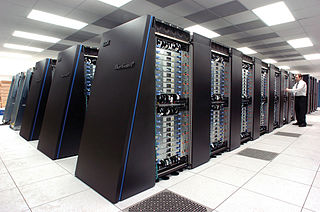
\includegraphics[width=\textwidth]{img/hpc.jpg}
        \caption{Actually this}
        \label{fig:my_label}
    \end{figure}
    \end{column}
\end{columns}
\end{frame}
\note{ I won't go into too much detail here as James will be giving a talk next week on this, however, what this means is that we have a system that has a lot of RAM that we can use as storage for running our Ceph instance}

\begin{frame}{Cluster - Deploying Ceph}
 \begin{figure}
     \centering
     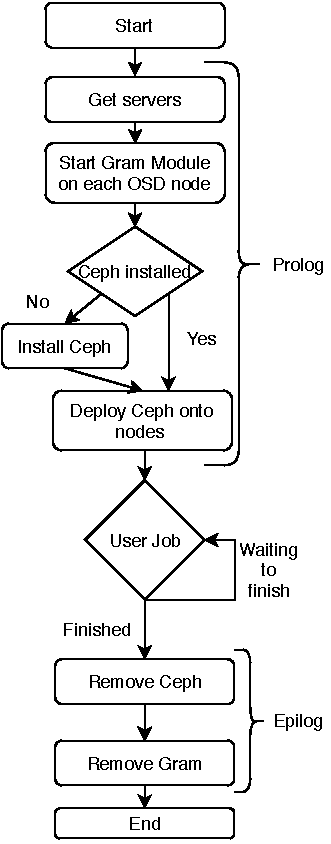
\includegraphics[width=\textwidth,height=0.7\textheight,keepaspectratio]{img/UGECeph.pdf}
     \caption{Deploy Script}
     \label{fig:my_label}
 \end{figure}
\end{frame}
\note{Walk through Script}